\documentclass[a4paper,12pt]{article} % тип документа

\usepackage{tabto}
\usepackage{graphicx}
\usepackage{wrapfig}

\usepackage{pgfplots}

\usepackage[%
    left=0.60in,%
    right=0.60in,%
    top=1.0in,%
    bottom=1.0in,%
    paperheight=11in,%
    paperwidth=8.5in%
]{geometry}%

\usepackage{hyperref}
\usepackage[rgb]{xcolor}

%  Русский язык

\usepackage[T2A]{fontenc}			% кодировка
\usepackage[utf8]{inputenc}			% кодировка исходного текста
\usepackage[english,russian]{babel}	% локализация и переносы


% Математика
\usepackage{amsmath,amsfonts,amssymb,amsthm,mathtools} 


\usepackage{wasysym}

\author{Платонов Е. Р. Б04-301}
\title{\textbf{1.1.1 Измерение удельного сопротивления нихромовой проволоки}}
\date{\today}
\begin{document}
\maketitle

\section{Аннотация}
\tabВ работе измеряется удельное сопротивление тонкой проволоки круглого сечения, изготовленной из нихромового сплава. Используются следующие методы измерений сопротивления:

1) определение углового коэффициента наклона зависимости напряжения на проволоке от тока 
через неё, измеряемых с помощью аналоговых и цифровых вольтметров и амперметров

2) измерение с помощью моста постоянного тока. Геометрические размеры образца измеряются с 
помощью линейки, штангенциркуля и микрометра. Детально исследуется систематические и 
случайные погрешности проводимых измерений.

\section{Теоретические сведения}

\begin{wrapfigure}{L}{0.4\textwidth}
\centering
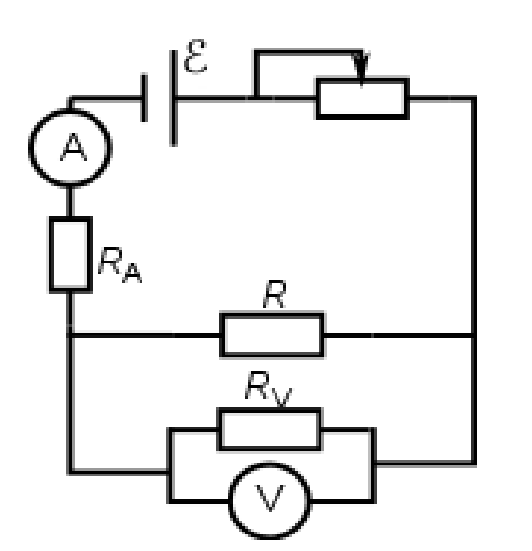
\includegraphics[width=0.35\textwidth]{imgs/схема1.png}
\caption{\label{схема}Схема установки}
\end{wrapfigure}

\tabУдельное споротивление однородной проволоки круглого сечения:
\begin{equation}\label{удсоп}
\rho=R\frac{\pi d^2}{4l},
\end{equation}
где $R$ - сопротивление проволоки, $l$ - длина, $d$ - диаметр сечения проволоки.

Согласно закону Ома напряжение $V$ и ток $I$ в образце связаны соотношением:
\begin{equation}
V=RI
\end{equation}

Для измерения напряжения и тока использовалась схема рис. 1.
Ввиду неидеальности используемого вольтметра необходимо 
учесть поправку на его конечное сопротивление $R_V$. Показания амперметра $I_A$ и вольтметра $V_B$ связаны соотношением:
\begin{equation}
V_B=R'I_A,
\end{equation}
\tabГде $R'$ -- сопротивление параллельно соединенных проволоки и 
вольтметра, причём $\frac{1}{R'}=\frac{1}{R}+\frac{1}{R_V}$
График зависимости $V_B$($I_A$) должен представлять прямую, угловой коэффициент которой есть $R'$, откуда сопротивление образца может быть найдено как:

\begin{equation}
    R = \frac{R_VR'}{R_V-R'} = \frac{R'}{1-\frac{R'}{R_V}}
\end{equation}

\section{Оборудование и инструментальные погрешности}
\tab\textbf{Линейка} : $\Delta_{\text{лин}} = \pm 0,5$ мм (по цене деления). 

\textbf{Штангенциркуль}: $\Delta_{\text{шт}} = \pm 0,05$ мм (маркировка производителя)

\textbf{Микрометр} : $\Delta_{\text{мкм}} = \pm 0,01$ мм (маркировка производителя)

\textbf{Вольтметр} :
\begin{table}[h]
\centering
\caption{Характеристики вольтметра}
\begin{tabular}{|c|c|}
\hline 
Система & Магнитно-электрическая \\ 
\hline 
Класс точности & 0,5 \\ 
\hline 
Шкала & линейная, 150 делений  \\ 
\hline 
Предел измерений & 0,75 В \\ 
\hline 
Цена деления & 5 мВ \\ 
\hline 
Внутреннее сопротивление & 5 кОм \\ 
\hline 
Погрешность при считывании со шкалы & $\pm 2,5$ мВ \\ 
\hline 
Макс. погрешность & $\pm3,75$ мВ \\ 
\hline 
\end{tabular} 
\end{table}

\textbf{Амперметр} :
\begin{table}[h]
\centering
\caption{Характеристики амперметра}
\begin{tabular}{|c|c|}
\hline 
Система & Цифровая \\  
\hline 
Разрядность дисплея & 5 ед. \\ 
\hline 
Внутреннее сопротивление & 1,2 Ом \\ 
\hline 
Погрешность & $\pm (0,002X+0,02)$ мА \\ 
\hline 
\end{tabular} 
\end{table}

\textbf{Мост постоянного тока P4833} :
\begin{table}[h]
\centering
\caption{Характеристики амперметра}
\begin{tabular}{|c|c|}
\hline 
Класс точности & 0,1 \\  
\hline 
Разрядность магазина сопротивлений & 5 ед. \\ 
\hline 
Используемый диапазон измерений & $10^{-4}$ -- 10 Ом \\ 
\hline 
Погрешность в используемом диапазоне & $\pm 0,01$ Ом \\ 
\hline 
\end{tabular} 
\end{table}

Поскольку в нашем диапазоне измерения сопротивление проволоки во много раз меньше внутреннего сопротивления вольтметра, можно предположить, что $R=R'$ (из уравнения 4).

\section{Результаты измерений и обработка данных}
\subsection{Измерение диаметра проволоки}
\tabИзмерения проводились штангенциркулем и микрометром многократно на разных участках проволоки. Для каждого измерения штангенциркулем получено 0,35 мм. Результаты измерения микрометром представлены в таблице \ref{d_ism}.

\begin{table}[!ht]
    \caption{Измерения диаметра сечения проволоки микрометром}
    \label{d_ism}
    \centering
    \begin{tabular}{|l|l|l|l|l|l|l|l|l|l|l|}
    \hline
        N изм. & 1 & 2 & 3 & 4 & 5 & 6 & 7 & 8 & 9 & 10 \\ \hline
        d, мм & 0,365 & 0,36 & 0,37 & 0,37 & 0,37 & 0,365 & 0,36 & 0,365 & 0,36 & 0,365 \\ \hline
    \end{tabular}
\end{table}

Средний диаметр сечения: $\overline{d} = \frac{1}{N}\sum d_i$ = 0,3645 мм

Стандартное отклонение: $\sigma_d = \sqrt{\frac{1}{N-1}\sum(d_i-\overline{d})^2}$ = 0,004 мм

Случайная погрешность среднего: $\sigma_{\overline{d}} = \frac{\sigma_d}{\sqrt{N}}$ = 0,001 мм

С учётом инструментальной погрешности $\Delta_\text{мкм}$ = 0,01 мм погрешность измерения диаметра может быть вычислена как $\sigma_{\overline{d}}^\text{полн} = \sqrt{\sigma_{\overline{d}}^2+\Delta_\text{мкм}^2} \approx$ 0,0101 мм
\begin{center}
    Окончательные результаты измерения диаметра проволоки:\\
    Штангенциркулем: $d=0,35 \pm 0,05$ мм\\
    Микрометром: $d=0,3645 \pm 0,0101$ $(\varepsilon_d = 2,8 \%)$ мм\\ 
\end{center}

\subsection{Измерения сопротивления проволоки}
\tabРезультаты измерений напряжения и силы тока в зависимости от длины исследуемого образца проволоки представлены в таблице \ref{вахтабл} и на графике (рис. \ref{графики})
\begin{table}[!ht]
    \label{вахтабл}
    \caption{Зависимость $V_B$ от $I_A$ для разных длин проволоки $l$}
    \centering
    \begin{tabular}{|l|l|l|l|l|l|l|l|l|l|l|l|l|}
    \hline
        ~ & \multicolumn{10}{|c|}{$l = 50 \pm$ 0,05 см $(\sigma_l = 0,1 \%)$}\\ \hline
        $V_B$, мВ & 585 & 495 & 450 & 415 & 370 & 350 & 650 & 710 & 610 & 625\\ \hline
        $I_A$, мА & 114,67 & 96,35 & 87,07 & 80,33 & 71,57 & 68,21 & 126,6 & 138,25 & 119,75 & 121,74\\ \hline
        ~ & \multicolumn{10}{|c|}{$l = 30 \pm$ 0,05 см $(\sigma_l = 0,17 \%)$}\\ \hline
        $V_B$, мВ & 380 & 350 & 315 & 290 & 260 & 690 & 625 & 560 & 510 & 450\\ \hline
        $I_A$, мА & 121,81 & 110,97 & 100,26 & 91,78 & 82,68 & 220,29 & 200,13 & 178,98 & 163,13 & 144,2\\ \hline
        ~ & \multicolumn{10}{|c|}{$l = 20 \pm$ 0,05 см $(\sigma_l = 0,25 \%)$}\\ \hline
        $V_B$, мВ & 260 & 265 & 305 & 340 & 370 & 430 & 480 & 220 & 190 & 155\\ \hline
        $I_A$, мА & 122,04 & 126,12 & 145,08 & 160,61 & 176,16 & 204,65 & 228,01 & 104,31 & 90,84 & 73,78\\ \hline
    \end{tabular}
\end{table}

\begin{figure}[h!]
\centering
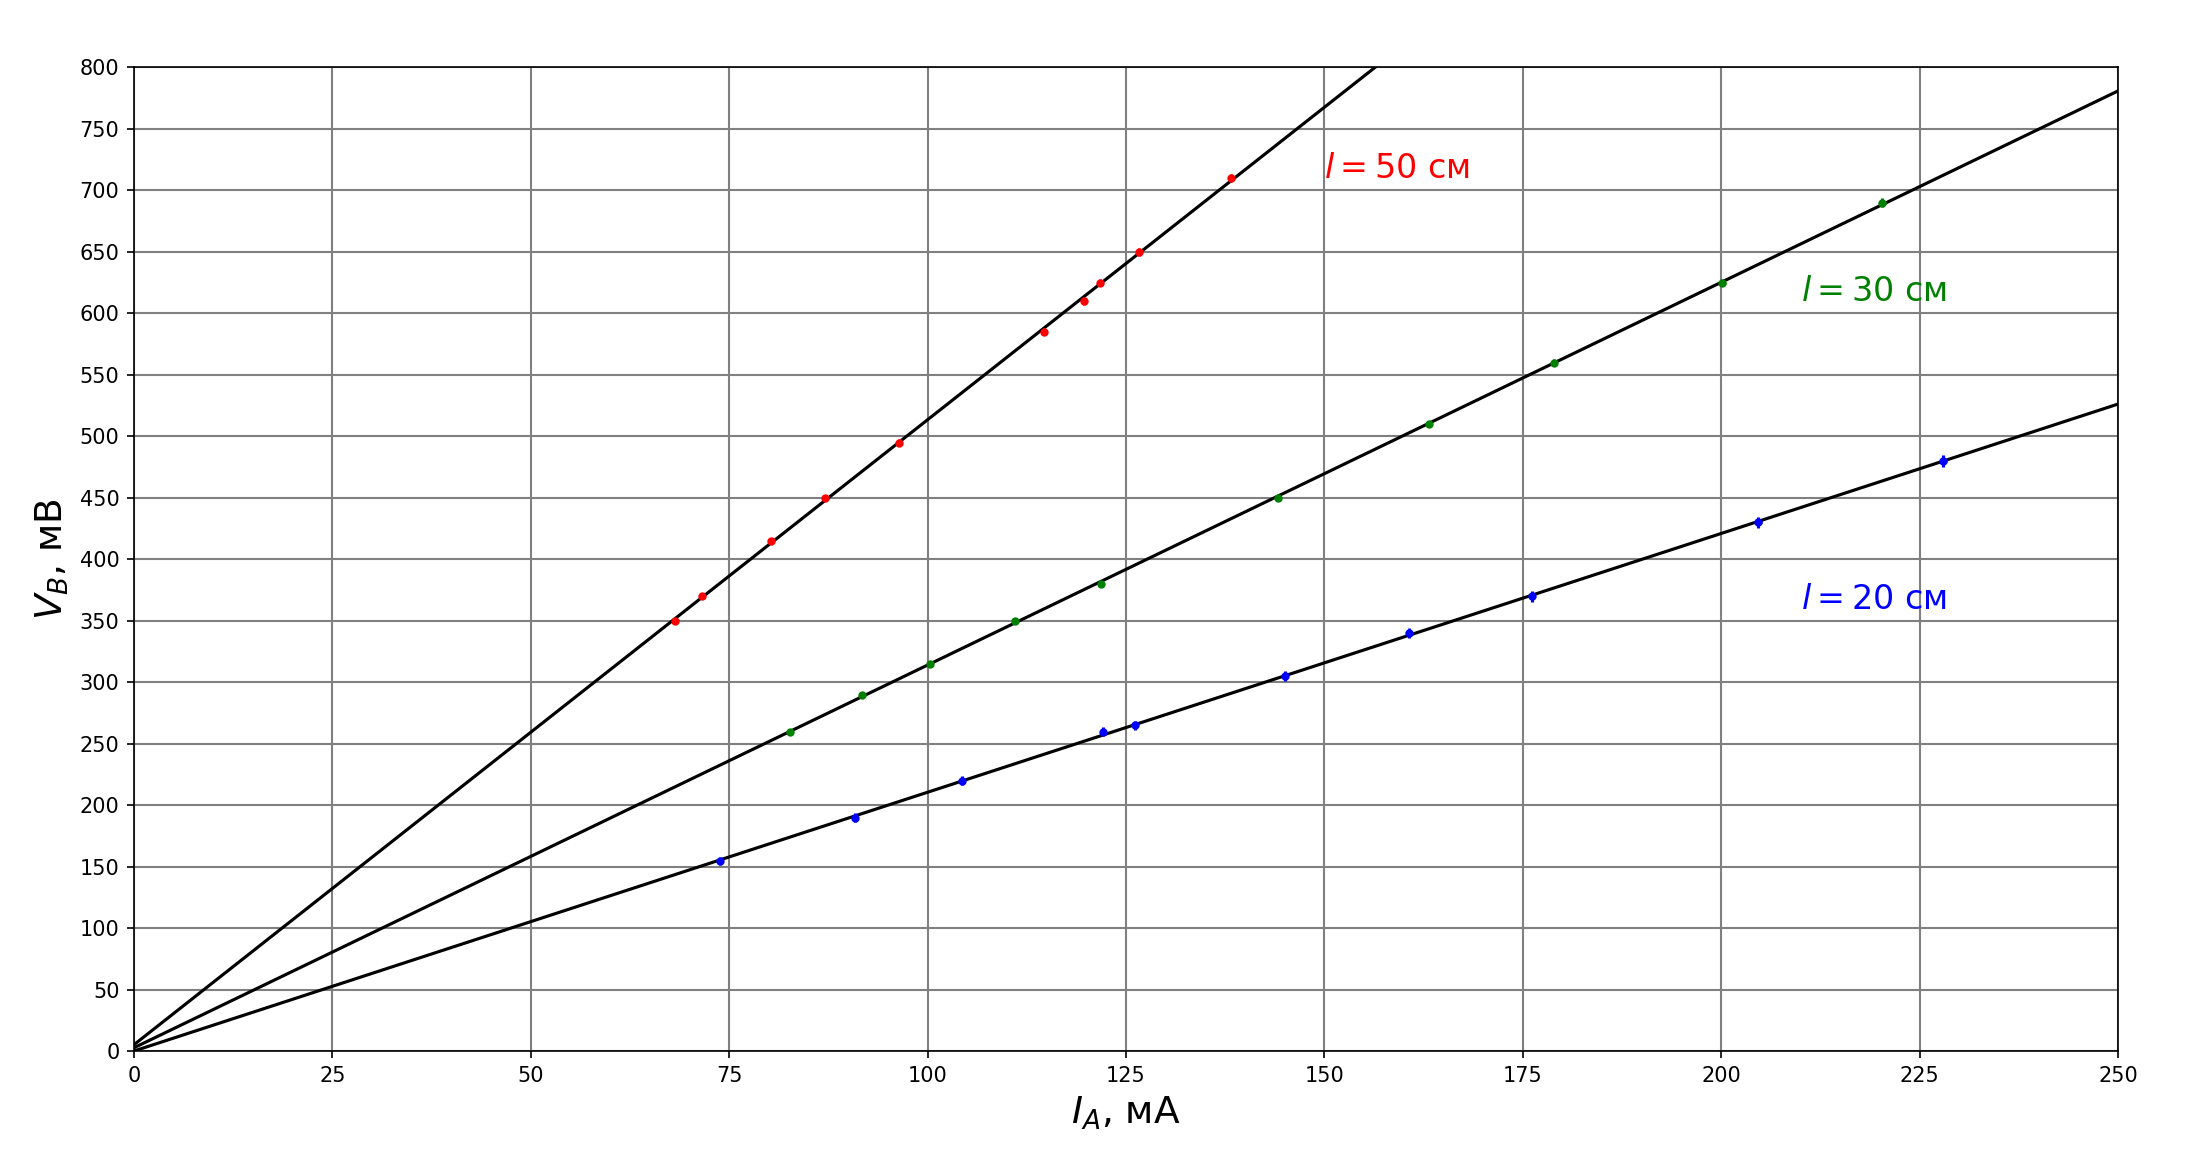
\includegraphics[width=\textwidth]{imgs/вах.png}
\caption{Результаты измерений напряжения $V$ (мВ) в зависимости от тока $I$ (мА) для проволок разной длины $l$ и их линейная аппроксимация } 
\label{графики}
\end{figure}

Для каждой длины $ l $ проводим расчет $\overline{R}$ методом наименьших квадратов для прямой, проходящей через начало координат (используется Python). Найдем случайную ошибку измерения по формуле:
\begin{equation}
\sigma_{R}^{\text{сл}} = \sqrt{\frac{1}{N(N-1)}\sum \left( \frac{V_i}{I_i}-\overline{R} \right)^2}
\end{equation}
\tabОценим возможную систематическую погрешность, обусловленную инструментальными 
погрешностями приборов. Предполагая, что при всех измерениях относительная погрешность 
приборов одинакова, оценим погрешность вычисления частного $R$ = $V/I$ при максимальных 
значениях $V$ и $I$:
\begin{equation}
\frac{\Delta_{R}^{\text{сист}}}{R}=\sqrt{\left( \frac{\Delta_V}{V} \right)^2+\left( \frac{\Delta_I}{I} \right)^2}
\end{equation}
Полная погрешность $R$:
\begin{equation}
    \sigma_{{R}}^\text{полн} = \sqrt{(\sigma_{R}^\text{сл})^2+(\Delta_R^{\text{сист}})^2}
\end{equation}

\begin{table}[h]
\centering
\caption{Результаты измерения сопротивления проволок}
\begin{tabular}{|c|c|c|c|c|c|c|}
\hline 
$l, $см & $\overline{R}$, Ом & $\sigma_{R}^{\text{сл}}$, Ом & $\Delta_{R}^{\text{сист}}$, Ом & $\sigma_{R}$, Ом & $R$, Ом & $R_\text{мост}$, Ом\\ 
\hline 
20 & 2,1 & 0,0315 & 0,018 & 0,036 & 2,1$\pm$ 0.036 $(\varepsilon_R = 1,7\%)$& $2,19 \pm 0,01$\\ 
\hline 
30 & 3,13 & 0,0817 & 0,027 & 0,086 & 3,13$\pm$  0.086 $(\varepsilon_R = 2,7\%)$ & $3,31 \pm 0,01$\\ 
\hline 
50 & 5,14 & 0,1851 & 0,044 & 0,19 & 5,14$\pm$ 0.19 $(\varepsilon_R = 3,7\%)$ & $5,36 \pm 0,01$\\ 
\hline 
\end{tabular} 
\label{сопротив}
\end{table} 

\subsection{Измерение удельного сопротивления проволоки}
\tabПо формуле (1) находим удельное сопротивление материала проволоки, используя значения 
$R$, полученные п. 4.2.

Погрешноть удельного сопротивления посчитаем по формуле:
\begin{equation}
\sigma_{\rho} = \rho\sqrt{\left( \frac{\sigma_R}{R} \right)^2+\left( 2\frac{\sigma_d}{d} \right)^2+\left( \frac{\sigma_l}{l} \right)^2}
\end{equation}

\begin{table}[h!]
\caption{Результаты измерения $\rho$ для каждой из длин проволок}
\centering
\begin{tabular}{|c|c|c|}
\hline 
$l$, см & $\rho$, $10^{-6}$ Ом $\cdot$м &$\sigma_{\rho}$, $10^{-8}$Ом$\cdot$м \\ 
\hline 
20 & 1,096 & 6,36 \\ 
\hline 
30 & 1,089 & 6,44 \\ 
\hline 
50 & 1,073 & 6,79 \\ 
\hline 
\end{tabular} 
\label{удсопрот}
\end{table}

Усредняя результаты 3 опытов, окончательно получим:
\begin{equation}
    \overline{\rho} = (1,086 \pm 0,065)\cdot10^{-6} 
    \text{ Ом}\cdot\text{м } (\varepsilon_\rho = 6 \%)
\end{equation}

\newpage
\section{Вывод}
\tabВ работе получено значение удельного сопротивления образца нихромовой проволоки $(1,086\pm0,065)\cdot10^{-6}$ Ом$\cdot$м. Табличное значение варьируется от 0,97 $\cdot10^{-6}$ Ом$\cdot$м до 1,12 $\cdot10^{-6}$ Ом$\cdot$м. Это означает, что схема представленная в работе позволяет с высокой точностью определить удельное сопротивление проволоки.

Наибольший вклад в погрешность удельного сопротивления внесла погрешность микрометра, которая из-за возвендения в квадрат удваивается и составляет 5,6\%. Также, погрешность измерения сопроивления была бы меньше, если бы в работе использовался не аналоговый, а цифровой вольтметр, так как, при считывании показаний со шкалы, возникает неточность, связанная как с городской тряской, так и с неидеальностью человеческого зрения.
\end{document}
